\section{Zielsetzung}
\label{sec:Zielsetzung}
In diesem Versuch soll die Wellenlänge eines Lasers mit Hilfe des Michelson-Interferometers bestimmt werden.
Mit selbigem Versuchsaufbau ist weiter der Brechungsindex von Luft zu bestimmen.

\section{Theorie}
\label{sec:Theorie}
Um den Aufbau und die Funktionsweise des Michelson-Interferometeres zu erläutern, 
sind eine Vorkenntnisse und Bedingungen, die getroffen werden müssen, nötig. Diese 
werden im Folgenden betrachtet.

\subsection{Interferenz und Kohärenz von Licht}
Licht ist eine elektromagnetische Welle, deren Ausbreitung sich mit den Maxwell-Gleichungen
beschreiben lässt. Im Allgemeinen lässt sich die orts- und zeitabhängige ($x,t$) elektrische Feldstärke einer solchen Welle mit

\begin{align}
\vec{E}(x,t) = \vec{E_\text{0}} \cos(kx - \omega t - \delta)
\end{align}

darstellen, wobei $k = \frac{2\pi}{\lambda}$ die Wellenzahl mit $\lambda$ als Wellenlänge, $\omega$ die Kreisfrequenz
und $\delta$ einen beliebigen Phasenwinkel repräsentieren. Für solche Gleichungen gilt das Superpositionsprinzip,
sodass sich zwei (oder mehr) an einem Ort $P$ ankommende Wellen überlagern und die Feldstärke addiert werden kann.
Da sich aufgrund der hohen Frequenz der genutzten Lichtquelle allerdings besser die Lichtintensität 

\begin{align*}
I = \mathrm{const} |\vec{E}|^{2}
\end{align*}

beobachten lässt, ergibt sich für die Addition zweier Wellen

\begin{align}
I_\text{ges} = 2 \mathrm{const} \vec{E_\text{0}}^{2} (1 + \cos(\delta_\text{2} - \delta_\text{1})).
\end{align}

\noindent Hierbei wird deutlich, dass der zweite Teil der Summe, welcher Interferenzterm genannt wird, abhängig von der
Phasenbeziehung $(\delta_\text{2} - \delta_\text{1})$ ist und somit Werte von $-2 \mathrm{const} \vec{E_\text{0}}^{2}$ bis 
$2 \mathrm{const} \vec{E_\text{0}}^{2}$ annehmen kann. Insbesondere verschwindet er bei einer Phasenverschiebung von einem
ungeraden Vielfachen von $\pi$. Aufgrund der statistischen Natur der Entstehung von Licht lässt sich somit aus Licht
zweier verschiedener Lichtquellen im Allgemeinen keine Interferenz beobachten. Es wird von inkohärentem Licht gesprochen.
Kohärentes Licht, welches beispielsweise mit einem Laser erzeugt werden kann, besitzt gemäß Gleichung (1) ein festes $k$, 
$\omega$ und $\delta$ für alle emittierten Wellenzüge. Wird kein Laser, sondern eine konventionelle Lichtquelle verwendet,
sind eine Bedingungen für eine Kohärenz gegeben. Wichtig ist die Kohärenzlänge 
\begin{align}
l = N \lambda,
\end{align}
welche die maximale Länge entlang eines interferenzfähigen Wellenzuges beschreibt. Wird zudem die Ausbreitungsgeschwindigkeit 
zweier Teilbündel betrachtet und mithilfe einer Fouriertransformation die Breite der Beugungsmaxima bestimmt,
folgt für diese
\begin{equation*}
  \Delta \lambda = \frac{\lambda_\text{0}^{2}}{c \tau}.
\end{equation*}
Die Kohärenzzeit ist demnach
\begin{equation*}
  \tau = \frac{l}{c},
\end{equation*}
womit sich
\begin{equation}
  \Delta \lambda = \frac{\lambda_\text{0}^{2}}{l}
\end{equation}
ergibt.
Für eine reelle, ausgedehnte Lichtquelle sind entweder die Ausdehnung oder der Öffnungswinkel einzuschränken, um Interferenzeffekte beobachten zu können,
da diese eine eigene Phasenverschiebung verursachen, welche die eigentlich zu beobachtbare Interferenz beeinträchtigt.
Abbildung \ref{fig:ausgedehnt} lässt sich die geometrische Beziehung
\begin{equation}
\Delta \phi = \frac{2\pi}{\lambda}a \sin(\gamma)
\end{equation}
entnehmen.
\begin{figure}
  \centering
  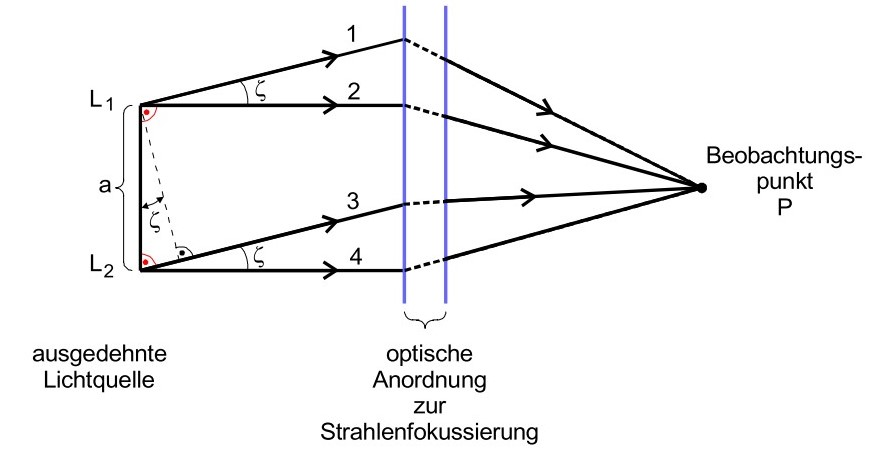
\includegraphics[scale=0.8]{ausgedehnt.jpg}
  \caption{Strahlengang einer ausgedehnten Lichtquelle \cite{Anleitung}.}
  \label{fig:ausgedehnt}
\end{figure}
Als Kohärenzbedingung für ausgedehnte Lichtquellen folgt aus der Bedingung $\Delta \phi \ll \pi$ die Ungleichung
\begin{equation}
  a \sin(\gamma) \ll \frac{\lambda}{2},
\end{equation}
sodass die Einschränkung des Öffnungswinkels leicht durch einen großen Abstand zur Lichtquelle realisiert werden kann.

\subsection{Das Michelson-Interferometer}
\begin{figure}[H]
  \centering
  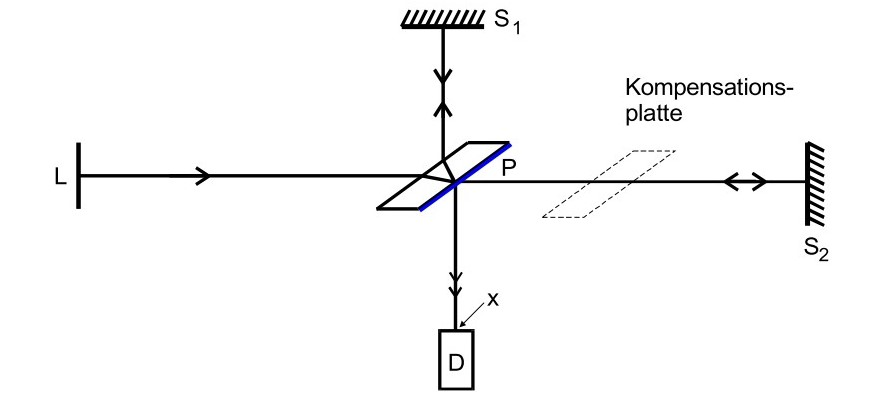
\includegraphics[scale=0.7]{Schema.jpg}
  \caption{Schematischer Aufbau eines Michelson-Interferometers \cite{Anleitung}.}
  \label{fig:schema}
\end{figure}
Beim Michelson-Interferometer wird mittels eines semipermeablen Materials ein Lichtstrahl in zwei Bündel geteilt, welche
reflektiert und zusammengeführt werden, um optische Messungen durchzuführen. 
Der Weg eines der beiden Lichtbündel wird hierbei so beeinflusst, dass bei deren
Zusammenführung Interferenzeffekte zu beobachten sind. Es ist zu beachten, dass systematische Unterschiede der Weglänge der
Lichtbündel unter Berücksichtigung der Kohärenzlänge ausgeglichen werden müssen, sodass eine Kompensationsplatte in den Weg eines der Bündel gesetzt werden muss (s. Abbildung \ref{fig:schema}),
da der Strahl zu $S_1$ die Platte $P$ dreimal durchläuft, der Strahl zu $S_2$ allerdings nur einmal. Bei gleichen Längen 
$\overline{S_1 P}$ und $\overline{S_2 P}$ ergibt sich so beim Detektor $D$ ein Gangunterschied von $\frac{\lambda}{2}$, welcher
destruktive Interferenz hervorruft. \\
Wird nun ein Spiegel um die Strecke $\Delta d$ verschoben, so ändert sich die Intensität des Lichts am Ort $D$.
Aufgrund dieser Tatsache lässt sich mit dem abgebildeten Aufbau die Wellenlänge $\lambda$ des verwendeten Lichts bestimmen,
da der Zusammenhang
\begin{align}
\Delta d = z \cdot \frac{\lambda}{2}
\end{align}
ersichtlich ist, wobei $z$ die Anzahl der während der Verschiebung beobachteten Interferenzmaxima darstellt. \\
Auch das Durchlaufen eines Mediums mit anderem Brechungsindex $n$ führt zu einer Änderung des Gangunterschieds (s. Abbildung \ref{fig:brechzahl}), welches
auf dieselbe Weise zu erkennen ist. 
\begin{figure}
  \centering
  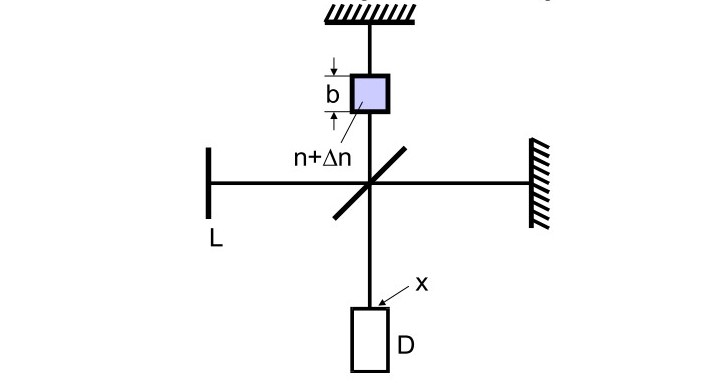
\includegraphics[scale=0.7]{Brechzahl.jpg}
  \caption{Schematischer Aufbau zur Messung von Brechungsindexunterschieden \cite{Anleitung}.}
  \label{fig:brechzahl}
\end{figure}
Ist die Strecke $b$, welche das Lichtbündel durch das Medium hindurch passiert, bekannt,
lässt sich somit auch der Brechungsindex von diesem bestimmen. Der optische Wegunterschied ergibt sich zu $\Delta n b$.
Wird dieser nun durch Veränderung des Drucks in dem Medium erhöht, so lassen sich während dieses Vorgangs 
erneut $z$ Interferenzmaxima beobachten, woraus die Beziehung 
\begin{align}
 b \cdot \Delta n = \frac{z \lambda}{2}
\end{align}
folgt. \\
Weiterhin wird angenommen, dass es sich in den hier verwendeten Durckbereichen um ideale Gase handelt, für die die Näherung
\begin{align}
n = 1 + \frac{f}{2} N
\end{align}
genutzt wird, wobei $N$ die Anzahl der durch Lichtwellen zur Schwingung angeregten Moleküle pro Volumeneinheit bezeichnet.
Dementsprechend ist die Anzahl der Moleküle bei gegebenem Druck $p$ und Temperatur $T$ gegeben durch
\begin{align*}
N(p,T) &= \frac{p}{T}\frac{T_0}{p_0}N_\text{L},  
\end{align*}
wobei $N_\text{L}$ die Loschmidtsche Zahl ist und $p_\text{0}$ sowie $T_\text{0}$ die Normalbedingungen sind.
Damit ergibt sich für die Differenz der Brechungsindizes $\Delta n$ die Formel
\begin{align}
\Delta n(p,p') = \frac{f}{2}N_L\frac{T_0}{p_0}\frac{1}{T}(p-p').
\end{align}
Unter Normalbedingungen folgt
\begin{align}
  n(p_0,T_0) = 1 + \Delta n(p,p')\frac{T}{T_0}\frac{p_0}{\Delta p}.
\end{align}